\documentclass[12pt]{article}
\usepackage[utf8]{inputenc}
\usepackage{ctex}
\usepackage{booktabs} % 用于绘制三线表
\usepackage{geometry}
\usepackage{graphicx}
\usepackage{longtable} % 用于绘制跨页长表格
\geometry{a4paper, margin=1in}
\usepackage{caption}

\title{皮安表电流测量完整数据记录}
\author{}
\date{\today}

\begin{document}

\maketitle

\section*{实验数据}
以下表格记录了皮安表的实时电流测量数据。视频前20秒为仪器量程调整阶段，有效稳定测量从视频 00:21 开始。我们将 00:21 定义为初始时间 $t = 0$ 秒，采样间隔为 $\Delta t = 5$ 秒，单位为纳安（nA）。记录直至视频 08:56 屏幕变暗前的最后有效读数。

\begin{table}[ht]
\centering
\caption{随时间变化的电流测量值（含拟合预测至900s）}
\label{tab:current_data}
\resizebox{\textwidth}{!}{
\begin{tabular}{cc|cc|cc|cc|cc|cc}
\toprule
时间(s) & 电流(nA) & 时间(s) & 电流(nA) & 时间(s) & 电流(nA) & 时间(s) & 电流(nA) & 时间(s) & 电流(nA) & 时间(s) & 电流(nA) \\
\midrule
0 & 3.9724 & 155 & 3.7684 & 310 & 3.4998 & 465 & 3.2339 & 620 & 2.8453 & 775 & 2.3897 \\
5 & 3.9167 & 160 & 3.7652 & 315 & 3.4923 & 470 & 3.2261 & 625 & 2.8318 & 780 & 2.3737 \\
10 & 3.9209 & 165 & 3.7639 & 320 & 3.4867 & 475 & 3.2189 & 630 & 2.8182 & 785 & 2.3577 \\
15 & 3.9072 & 170 & 3.7624 & 325 & 3.4803 & 480 & 3.2064 & 635 & 2.8045 & 790 & 2.3416 \\
20 & 3.8943 & 175 & 3.7645 & 330 & 3.4712 & 485 & 3.1977 & 640 & 2.7907 & 795 & 2.3255 \\
25 & 3.8844 & 180 & 3.7646 & 335 & 3.4656 & 490 & 3.1919 & 645 & 2.7768 & 800 & 2.3092 \\
30 & 3.8798 & 185 & 3.7651 & 340 & 3.4554 & 495 & 3.1839 & 650 & 2.7629 & 805 & 2.2929 \\
35 & 3.8753 & 190 & 3.7670 & 345 & 3.4457 & 500 & 3.1754 & 655 & 2.7489 & 810 & 2.2765 \\
40 & 3.8854 & 195 & 3.7711 & 350 & 3.4389 & 505 & 3.1656 & 660 & 2.7348 & 815 & 2.2601 \\
45 & 3.8869 & 200 & 3.7718 & 355 & 3.4304 & 510 & 3.1567 & 665 & 2.7207 & 820 & 2.2435 \\
50 & 3.8793 & 205 & 3.7684 & 360 & 3.4253 & 515 & 3.1432 & 670 & 2.7064 & 825 & 2.2269 \\
55 & 3.8706 & 210 & 3.7613 & 365 & 3.4199 & 520 & 3.0999 & 675 & 2.6921 & 830 & 2.2102 \\
60 & 3.8600 & 215 & 3.7517 & 370 & 3.4093 & 525 & 3.0879 & 680 & 2.6777 & 835 & 2.1934 \\
65 & 3.8475 & 220 & 3.7384 & 375 & 3.4014 & 530 & 3.0759 & 685 & 2.6633 & 840 & 2.1765 \\
70 & 3.8363 & 225 & 3.7258 & 380 & 3.3931 & 535 & 3.0637 & 690 & 2.6487 & 845 & 2.1596 \\
75 & 3.8367 & 230 & 3.7090 & 385 & 3.3842 & 540 & 3.0515 & 695 & 2.6341 & 850 & 2.1426 \\
80 & 3.8360 & 235 & 3.6983 & 390 & 3.3753 & 545 & 3.0392 & 700 & 2.6194 & 855 & 2.1255 \\
85 & 3.8367 & 240 & 3.6817 & 395 & 3.3609 & 550 & 3.0268 & 705 & 2.6046 & 860 & 2.1083 \\
90 & 3.8360 & 245 & 3.6670 & 400 & 3.3520 & 555 & 3.0143 & 710 & 2.5898 & 865 & 2.0911 \\
95 & 3.8334 & 250 & 3.6465 & 405 & 3.3369 & 560 & 3.0018 & 715 & 2.5748 & 870 & 2.0738 \\
100 & 3.8281 & 255 & 3.6322 & 410 & 3.3294 & 565 & 2.9892 & 720 & 2.5598 & 875 & 2.0564 \\
105 & 3.8221 & 260 & 3.6155 & 415 & 3.3148 & 570 & 2.9765 & 725 & 2.5448 & 880 & 2.0389 \\
110 & 3.8165 & 265 & 3.5995 & 420 & 3.3060 & 575 & 2.9637 & 730 & 2.5296 & 885 & 2.0213 \\
115 & 3.8073 & 270 & 3.5849 & 425 & 3.2957 & 580 & 2.9509 & 735 & 2.5144 & 890 & 2.0037 \\
120 & 3.7902 & 275 & 3.5744 & 430 & 3.2877 & 585 & 2.9379 & 740 & 2.4990 & 895 & 1.9860 \\
125 & 3.7889 & 280 & 3.5617 & 435 & 3.2787 & 590 & 2.9249 & 745 & 2.4837 & 900 & 1.9682 \\
130 & 3.7957 & 285 & 3.5505 & 440 & 3.2711 & 595 & 2.9119 & 750 & 2.4682 &  &  \\
135 & 3.7904 & 290 & 3.5391 & 445 & 3.2619 & 600 & 2.8987 & 755 & 2.4526 &  &  \\
140 & 3.7847 & 295 & 3.5284 & 450 & 3.2551 & 605 & 2.8855 & 760 & 2.4370 &  &  \\
145 & 3.7786 & 300 & 3.5196 & 455 & 3.2489 & 610 & 2.8722 & 765 & 2.4213 &  &  \\
150 & 3.7731 & 305 & 3.5097 & 460 & 3.2418 & 615 & 2.8588 & 770 & 2.4055 &  &  \\
\bottomrule
\end{tabular}
}
\end{table}


\begin{figure}[htbp]
\centering
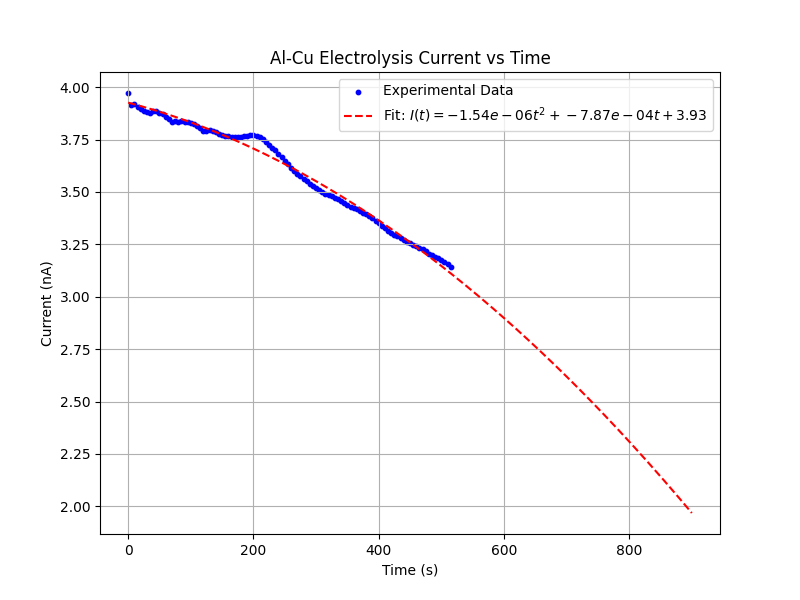
\includegraphics[width=0.8\textwidth]{fit_plot.png}
\caption{铝铜在纯水中电解随时间变化的电流及其拟合外推曲线}
\label{fig:fit_plot}
\end{figure}